\subsection{Etude de $\sum_{k=1}^n \frac{\ln(k)}{k}$ [Agro 2016]}

\begin{probleme}
On considère la suite $\suiteun{S}$ définie par :
$$\forall n\in \N^*, \quad S_n  =\sum_{k=1}^n \frac{\ln(k)}{k}$$

\begin{enumerate}
\item Etude de la nature de la suite $\suiteun{S}$.
\begin{enumerate}
\item Dresser le tableau  de variations de la fonction $x\mapsto \frac{\ln(x)}{x}$.
\item En déduire que, pour tout entier $k$ supérieur ou égal à $4$, on a : 
$$\int_k^{k+1} \frac{\ln(x)}{x}dx\leq \frac{\ln(k)}{k} \leq \int_{k-1}^{k} \frac{\ln(x)}{x}dx.$$
\item En déduire l'existence de trois constantes réelles positives, $A,B $ et $C$ telles que, pour tout entier naturel $n\geq 4$, on ait : 
$$\frac{\ln^2(n+1)}{2} -A\leq S_n-B \leq \frac{\ln^2(n)}{2} -C$$
\item En déduire la limite de la suite $\suiteun{S}$. 
\end{enumerate}
\item Recherche d'un éguivalent de $S_n$
\begin{enumerate}
\item Montrer que $\ln^2(n+1) \equivalent{n\tv \infty} \ln^2(n)$.
\item En déduire que $S_n\equivalent{n\tv \infty} \frac{\ln^2(n)}{2}$.
\end{enumerate}
\item Etude asymptotique de la suite $\suiteun{u}$ définie par : 
$$\forall n\in \N^*, \quad u_n=S_n -\frac{\ln^2(n)}{2}$$
\begin{enumerate}
\item Enoncer le théorème donnant la formule des accroissements finis (en particulier, on précisera avec soin les hypothèses de ce théorème).
\item A l'aide de la fonction $x \mapsto \ln^2(x) $   montrer que  pour tout $x\geq 3$
$$\ln^2(x+1) -\ln^2(x) \geq 2\frac{\ln(x+1)}{x+1}.$$
\item En déduire  que pour tout entier $n\geq 3$, $u_{n+1} -u_n \leq 0$.
\item En déduire que la suite $u$ converge. 
\end{enumerate}
\item Ecrire un script Python qui permet d'afficher les 20 premiers termes de la suite $\suite{S}$ sur un même graphique. 
\item Ecrire  un script Python qui permet d'afficher la fonction $x\mapsto \frac{\ln^2(x)}{x}$ sur l'intervalle $[1,20[$

 On pourra utiliser les bibliothéques pyplot et numpy importées de la manière suivante : 
\texttt{import maplotlib.pyplot as plt} et \texttt{import numpy as np}.
On rappelle l'utilisation des fonctions suivantes : 
\begin{itemize}
\item  Si $X$ et $Y$ sont deux listes (ou array numpy), lpya fonction \texttt{plt.plot(X,Y)} place les points dont les abscisses sont contenues dans X et les ordonnées dans Y et les relie entre eux par des segments. Si cette fonction n’est pas suivie de plt.show(), le graphique n’est pas affichés. 
\item \texttt{plt.plot(X,Y,o)}  Meme effet que plt.plot(X,Y) à la différence près que les points sont représentés par un symbole en forme de cercle et ne sont pas reliés. 
\item \texttt{np.arange(d,n,p)} permet de créer un tableau numpy allant de $d$ à $n$ (non inclus) par pas de $p$ 
\item \texttt{np.linspace(d,n,N)} permet de créer un tableau numpy de longueur $N$, espaçant linéairement les points de $d$ à $n$ ($n$ non inclus).
\end{itemize}
\end{enumerate}
\end{probleme}

%

\begin{correction}
\begin{enumerate}
\item \begin{enumerate}
\item Soit $f(x) = \frac{\ln(x)}{x}$, $f$ est définie et dérivable sur $\R_+^*$ et $$\forall x> 0, \quad  f'(x) = \frac{1 - \ln(x)}{x^2}$$

On a par ailleurs $\lim_{x\tv 0} f(x) = -\infty$ (ce n'est pas une forme indéterminée)  et $\lim_{x\tv +\infty } f(x) = 0$ par croissance comparée.

On a donc le tableau suivant : \\
\begin{center}
\begin{tikzpicture}
   \tkzTabInit{$x$ / 1 , $1-\ln(x)$ / 1, $x^2$ / 1, $f'(x)$/1, $f(x)$ /1.5 }{$0$, $e$, $+\infty$}
   \tkzTabLine{, +, z, -, }
      \tkzTabLine{, +, , +, }
            \tkzTabLine{, +, z, -, }
           
 \tkzTabVar{-/ $-\infty$, +/ $e^{-1}$, -/$0$ }
 \tkzTabIma{1}{3}{2}{  }
  % \tkzTabVal{1}{2}{0.5}{}{} 
\end{tikzpicture}
\end{center}

\item Pour tout $k\geq 3>e$  on  a pour tout $x\in [k,k+1] $
$$\frac{ln(x)}{x} \leq \frac{ln(k)}{k}$$
Donc en intégrant sur $[k,k+1]$ on obtient par positivité de l'intégrale: 
\begin{align*}
\int_k^{k+1} \frac{\ln(x)}{x} dx &\leq\int_k^{k+1}  \frac{\ln(k)}{k}dx\\
	\int_k^{k+1} \frac{\ln(x)}{x} dx &\leq  \frac{\ln(k)}{k}
\end{align*}

De même pour tout $k\geq 4>e+1$  on  a pour tout $x\in [k-1,k] $
$$\frac{\ln(k)}{k} \leq \frac{\ln(x)}{x}$$
Donc en intégrant sur $[k,k+1]$ on obtient par positivité de l'intégrale: 
\begin{align*}
\int_k^{k+1} \frac{\ln(k)}{k} dx &\leq\int_k^{k+1}  \frac{\ln(x)}{x}dx\\
\frac{\ln(k)}{k}&\leq  \int_k^{k+1}  \frac{\ln(x)}{x}dx\\
\end{align*}

On obtient bien les deux inégalités demandées. 
\item On somme maintenant la double inégalité pour $k$ variant de $4$ à $n$. On obtient : 
$$\begin{array}{rcl}
\ddp \sum_{k=4}^n\int_k^{k+1} \frac{\ln(x)}{x}dx\leq& \ddp \sum_{k=4}^n\frac{\ln(k)}{k} &\leq\ddp  \sum_{k=4}^n \int_{k-1}^{k} \frac{\ln(x)}{x}dx\\

\ddp \int_4^{n+1}\frac{\ln(x)}{x}dx&\ddp \leq S_n - \frac{\ln(3)}{3} - \frac{\ln(2)}{2}\leq & \ddp \int_{3}^{n} \frac{\ln(x)}{x}dx\\

\ddp \left[\frac{\ln^2(x)}{2}\right]_4^{n+1}\ddp \leq& S_n - \frac{\ln(3)}{3} - \frac{\ln(2)}{2}\leq & \ddp \left[\frac{\ln^2(x)}{2}\right]_3^n\\

\ddp\frac{\ln^2(n+1)}{2}- \frac{\ln^2(4)}{2}\ddp \leq& S_n - \frac{\ln(3)}{3} - \frac{\ln(2)}{2}\leq & \ddp \frac{\ln^2(n)}{2}-\frac{\ln^2(3)}{2}\\
\end{array}$$

On obtient l'inégalité voulue avec $A=\frac{\ln^2(4)}{2} = 2\ln^2(2)$, 
$B= \frac{\ln(3)}{3} + \frac{\ln(2)}{2}$
 et $C= \frac{\ln^2(3)}{2}$.
 \item $\lim_{n\tv +\infty} \frac{\ln^2(n+1)}{2} -A+B = +\infty$ donc 
 par  théorème de comparaison  
 $$\lim_{n\tv \infty} S_n = +\infty$$
\end{enumerate}
\item \begin{enumerate}
\item On considère le quotient des deux suites : 
\begin{align*}
\frac{\ln^2{n+1} }{\ln^2(n) } &= \frac{\ln^2(n(1+1/n)) }{\ln^2(n)} \\
										&=1+\frac{\ln^2(1+1/n)}{\ln^2(n)}
\end{align*}
Donc 
$$\lim_{n\tv +\infty } \frac{\ln^2{n+1} }{\ln^2(n) }= 1$$
on a bien 
 $$\ln^2(n+1) \equivalent{n\tv \infty} \frac{\ln^2(n)}{2}$$
\item On divise l'inégalité obentue en 2c) par $\ln^2(n)$
$$\frac{\ln^2(n+1)}{\ln^2(n)} -\frac{2A}{\ln^2(n)}\leq \frac{2S_n}{\ln^2(n)}-\frac{2B}{\ln^2(n)} \leq \frac{\ln^2(n)}{\ln^2(n)} -\frac{2C}{\ln^2(n)}$$
On a 
$$\lim_{n\tv +\infty} \frac{\ln^2(n+1)}{\ln^2(n)} -\frac{2A}{\ln^2(n)} = 1$$

$$\lim_{n\tv +\infty}-\frac{2B}{\ln^2(n)} = 0$$
et
$$\lim_{n\tv +\infty} \frac{\ln^2(n)}{\ln^2(n)} -\frac{2C}{\ln^2(n)}= 1$$
Le théorème des gendarmes assure que 
$$\lim_{n\tv +\infty}  \frac{2S_n}{\ln^2(n)}=1$$
c'est-à-dire $$S_n  \equivalent{n\tv \infty} \frac{\ln^2(n)}{2}$$
\end{enumerate}
\item Soit $(a,b) \in \R^2$ deux réels et $f $ une fonction continue sur $[a,b]$ et dérivable sur $]a, b[$, il existe alors $c\in ]a, b[$ tel que 
$$\frac{f(b)-f(a)}{b-a} =f'(c)$$
\item On applique le TAF sur $[x,x+1]$ avec $x\geq 3$. $x\mapsto \ln^2(x)$ est bien continue sur $[x,x+1]$ et dérivable sur $]x, x+1[$, ainsi il existe $c\in ]x, x+1[$ tel que 
$$\frac{\ln^2(x+1)-\ln^2(x)}{x+1-x} =2\frac{\ln(c)}{c}$$
Comme la fonction $f(x) =\frac{\ln(x)}{x}$ est décroissante sur $[e, +\infty[\subset [3, +\infty[$ on a pour $c\in ]x,x+1[$ :
$$2\frac{\ln(c)}{c} \geq 2\frac{\ln(x+1)}{x}$$
Finalement 
$$\ln^2(x+1)-\ln^2(x) \geq 2\frac{\ln(x+1)}{x+1}$$
\item
\begin{align*}
 u_{n+1}-u_n &= S_{n+1} -S_n -\frac{\ln^2(n+1)-\ln^2(n)}{2}\\
 					&= \frac{\ln(n+1)}{n+1}- \frac{\ln^2(n+1)-\ln^2(n)}{2}\\
 					&= \frac{1}{2} \left(  \frac{2\ln(n+1)}{n+1}- \ln^2(n+1)-\ln^2(n)  \right)\\
 					&\leq 0\quad \text{ d'après la question précédente}
\end{align*}
Donc $\suite{u}$ est décroissante à partir de $n\geq 3$. 
\item D'après 1c) on  a
$$S_n -\frac{\ln^2(n)}{2 }\geq \frac{\ln^2(n+1) }{2} - A +B -\frac{\ln^2(n)}{2 }$$
Or 
\begin{align*}
\ln^2(n+1)-\ln^2(n) =\ln^2\left(1+\frac{1}{n}\right)
\end{align*}
Donc $\lim_{n\tv +\infty }  \frac{\ln^2(n+1) }{2} - A +B -\frac{\ln^2(n)}{2 } = A-B$. Comme une suite convergente est minorée, la suite $ \frac{\ln^2(n+1) }{2} - A +B -\frac{\ln^2(n)}{2 }$ est minorée et a fortiori la suite $S_n -\frac{\ln^2(n)}{2 }$ est minorée. Elle est décroissante et minorée, elle converge. 


\end{enumerate}
\end{correction}